% Prof. Dr. Ausberto S. Castro Vera
% UENF - CCT - LCMAT - Curso de Ci\^{e}ncia da Computa\c{c}\~{a}o
% Campos, RJ,  2021
% Disciplina: Paradigmas de Linguagens de Programa\c{c}\~{a}o


\chapter{Ferramentas existentes e utilizadas}

Neste cap\'{\i}tulo devem ser apresentadas pelo menos DUAS (e no m\'{a}ximo 5) ferramentas consultadas e utilizadas para realizar o trabalho, e usar nas aplica\c{c}\~{o}es. Considere em cada caso:
\begin{itemize}
  \item Nome da ferramenta (compilador-interpretador)
  \item Endere\c{c}o na Internet
  \item Vers\~{a}o atual e utilizada
  \item Descri\c{c}\~{a}o simples (m\'{a}x 2 par\'{a}grafos)
  \item Telas capturadas da ferramenta
  \item Outras informa\c{c}\~{o}es
\end{itemize}

    \section{Node JS}
    A linguagem JavaScript não está mais atrelada somente ao navegador. Por isso, para utilizar a linguagem sem precisar recorrer a um Browser, utiliza-se o nodeJS. O NodeJS, conhecido apenas como Node, nada mais é do que o V8 (Engine do JavaScript no navegador Google Chrome) fora do Chrome. Sendo assim, para instalar o Node basta entrar em https://nodejs.org e baixar a versão desejada. 
    
\begin{figure}[H]
	\centering
	
\includegraphics[width=0.3\linewidth]{Pictures/NodeLogo}
	\caption{}
	\label{fig:nodelogo}
\end{figure}


    
    \subsection{NPM}
    
    
    \begin{figure}[H]
    	\centering
    	
\includegraphics[width=0.2\linewidth]{Pictures/Npm-logo.svg}
    	\caption{}
    	\label{fig:npm-logo}
    \end{figure}

    Um gerenciador de pacotes é uma ferramenta fundamental para o desenvolvimento de aplicações. Por ele é possível instalar diversas dependências necessárias para o funcionamento da aplicação e gerenciar os pacotes e suas versões que o programa irá utilizar. O NPM (Node Package Manager) é o gerenciador de pacotes mais utilizado para o JavaScript. 
    Na imagem abaixo, utilizei o NPM para baixar um pacote chamado "express".
    
    \begin{figure}[H]
    	\centering
    	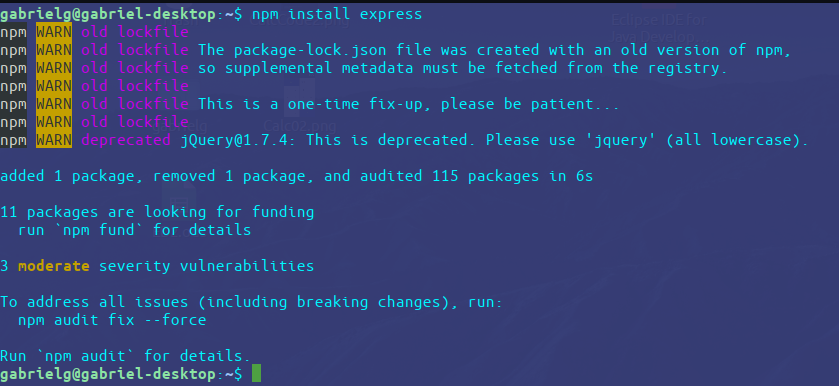
\includegraphics[width=0.7\linewidth]{Pictures/npm_express}
    	\caption{}
    	\label{fig:npmexpress}
    \end{figure}
	O NPM gera um arquivo chamado package.json. Este arquivo contém informações importantes do programa,como o nome, versão, arquivo inicial e suas dependências. Também é possível especificar certas condições nestes arquivos.
	\begin{figure}[H]
		\centering
		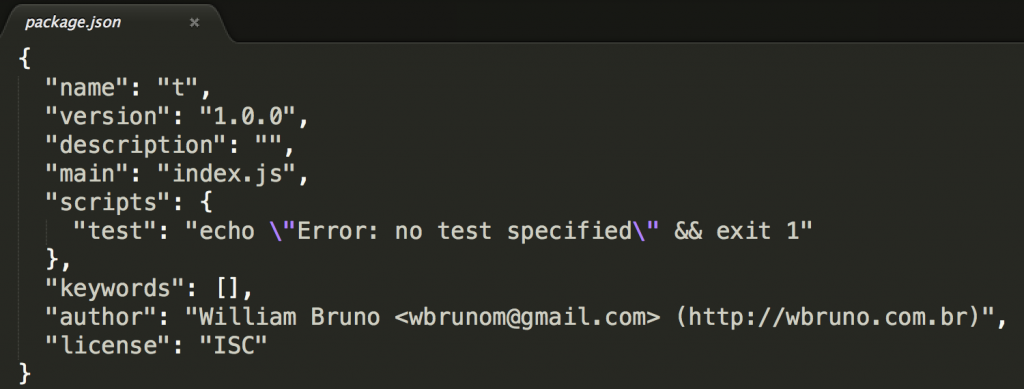
\includegraphics[width=0.7\linewidth]{Pictures/package-json}
		\caption{}
		\label{fig:package-json}
	\end{figure}
	
    
    

    
    \subsection{NVM}
    Devido a existência de várias versões do Node, o NVM - Node Version Manager - facilita o trabalho com versões diferentes. Por exemplo, se num projeto antigo decide-se pela versão 11.5, é possível com o NVM utilizar o node 11.5 sempre naquele projeto, mesmo após atualizar o node para versões mais recentes.
    Abaixo, utilizei o comando nvm ls, que lista todas as versões do node instaladas no computador. 
    
\begin{figure}[H]
	\centering
	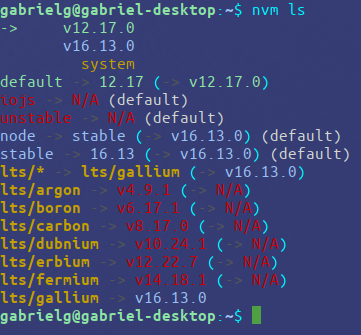
\includegraphics[width=0.6\linewidth]{Pictures/nvm_LS}
	\caption{}
	\label{fig:nvmls}
\end{figure}
    

	\section{IDEs}
	As Interfaces de Desenvolvimento Integrado, IDEs, são ferramentas importantes que auxiliam o programador a desenvolver aplicações fornecendo recursos, praticidade e dinamicidade. Imagine ter que escrever códigos enormes, acima de 200 linhas, num bloco de notas. Ou ter que navegar em arquivos e editá-los dentro de dezenas de diretórios e sub-diretórios sem nenhuma forma de visualizá-los. Seria uma tarefa extremamente árdua, e por isso, programar numa IDE poderosa permite a otimização do tempo de trabalho e fornece ganhos enormes de produtividade. Diversos recursos, como complemento de código e auto-importação de arquivos necessários, são apenas exemplos de formas que uma interface de desenvolvimento pode ajudar um programados.
	
    \subsection{Visual Studio Code}
    Nos dias atuais existem diversas versões de IDEs para as mais variadas linguagens de programação. Os exemplos vão desde o Netbeans e Eclipse para o Java ao Pycharm para o Python entre outras. IDEs feitas pensando especificamente em uma linguagem sempre tiveram vantagem em relação às IDEs multi-uso, como o sublime-text e o VS Code. Porém, atualmente este fato já não é mais realidade. Com o Visual Studio Code, que chamarei de VSC ou VS Code, programar em várias linguagens é fácil e dinâmico. 
    O VSC é uma IDE fácil de usar, relativamente leve e permite a instalação de inúmeras extensões para tornar o desenvolvimento o mais produtivo possível.
    Abaixo estão as extensões de JavaScript mais utilizadas:
    \begin{figure}[H]
    	\centering
    	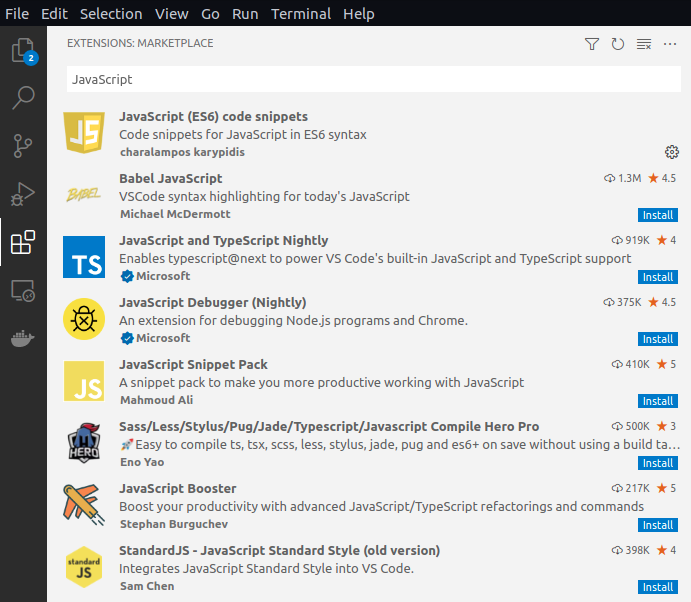
\includegraphics[width=0.7\linewidth]{Pictures/ExemplosExtensoes}
    	\caption{}
    	\label{fig:exemplosextensoes}
    \end{figure}
    
    Portanto, para programar em JavaScript, o VSCode é uma das melhores IDEs disponíveis. Além de permitir programar para web utilizando JS, HTML e CSS, também suporta outras linguages e tem suporte ao GitHUb.
     
    
    \begin{figure}[H]
    	\centering
    	
\includegraphics[width=0.2\linewidth]{Pictures/VSC_Logo}
    	\caption{}
    	\label{fig:vsclogo}
    \end{figure}
    
    \subsection{Webstorm}
    Embora seja pago, o Webstorm é uma excelente escolha na hora de desenvolver em JavaScript e TypeScript. O programa é desenvolvido pela JetBrains, uma empresa bem estabelecida no mercado de IDEs. PyCharm, IntelliJ entre outros são programas extremamente confiáveis e práticos desenvolvidos pela JetBrains.
    
	
\begin{figure}[H]
	\centering
	
\includegraphics[width=0.2\linewidth]{Pictures/WebStorm_Icon.svg}
	\caption{}
	\label{fig:webstormicon}
\end{figure}

	\subsection{Atom}
	\begin{figure}[H]
		\centering
		
\includegraphics[width=0.2\linewidth]{Pictures/Atom_1.0_icon}
		\caption{}
		\label{fig:atom1}
	\end{figure}
	O Atom é um programa leve, gratuito e prático de utilizar, assim como o VS Code. Tem integração com o GitHub e é ótimo para desenvolver em colaboração com outros desenvolvedores. É importante dizer que além disso, o Atom é open-source, assim como o VS Code.
	
	\begin{figure}[H]
		\centering
		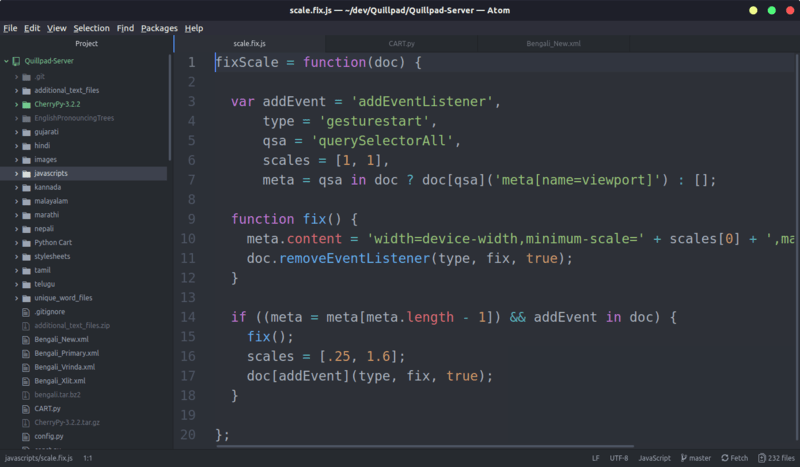
\includegraphics[width=0.7\linewidth]{Pictures/AtomIDE}
		\caption{}
		\label{fig:atomide}
	\end{figure}
	
	
	\subsection{JS Fiddle}
	\begin{figure}[H]
		\centering
		
\includegraphics[width=0.2\linewidth]{Pictures/JS_Fiddle}
		\caption{}
		\label{fig:jsfiddle}
	\end{figure}
	É importante mencionar também interpretadores e IDEs onlines que auxiliam no desenvolvimento de aplicações. Uma delas é o JS Fiddle. O JS Fiddle permite desenvolver, compartilhar e executar aplicações de forma simular à uma IDE padrão. Além disso, pela praticidade, pode ser uma alternativa para edição rápida em situações que configurar a interface de desenvolvimento não seja possível.

\begin{figure}[H]
	\centering
	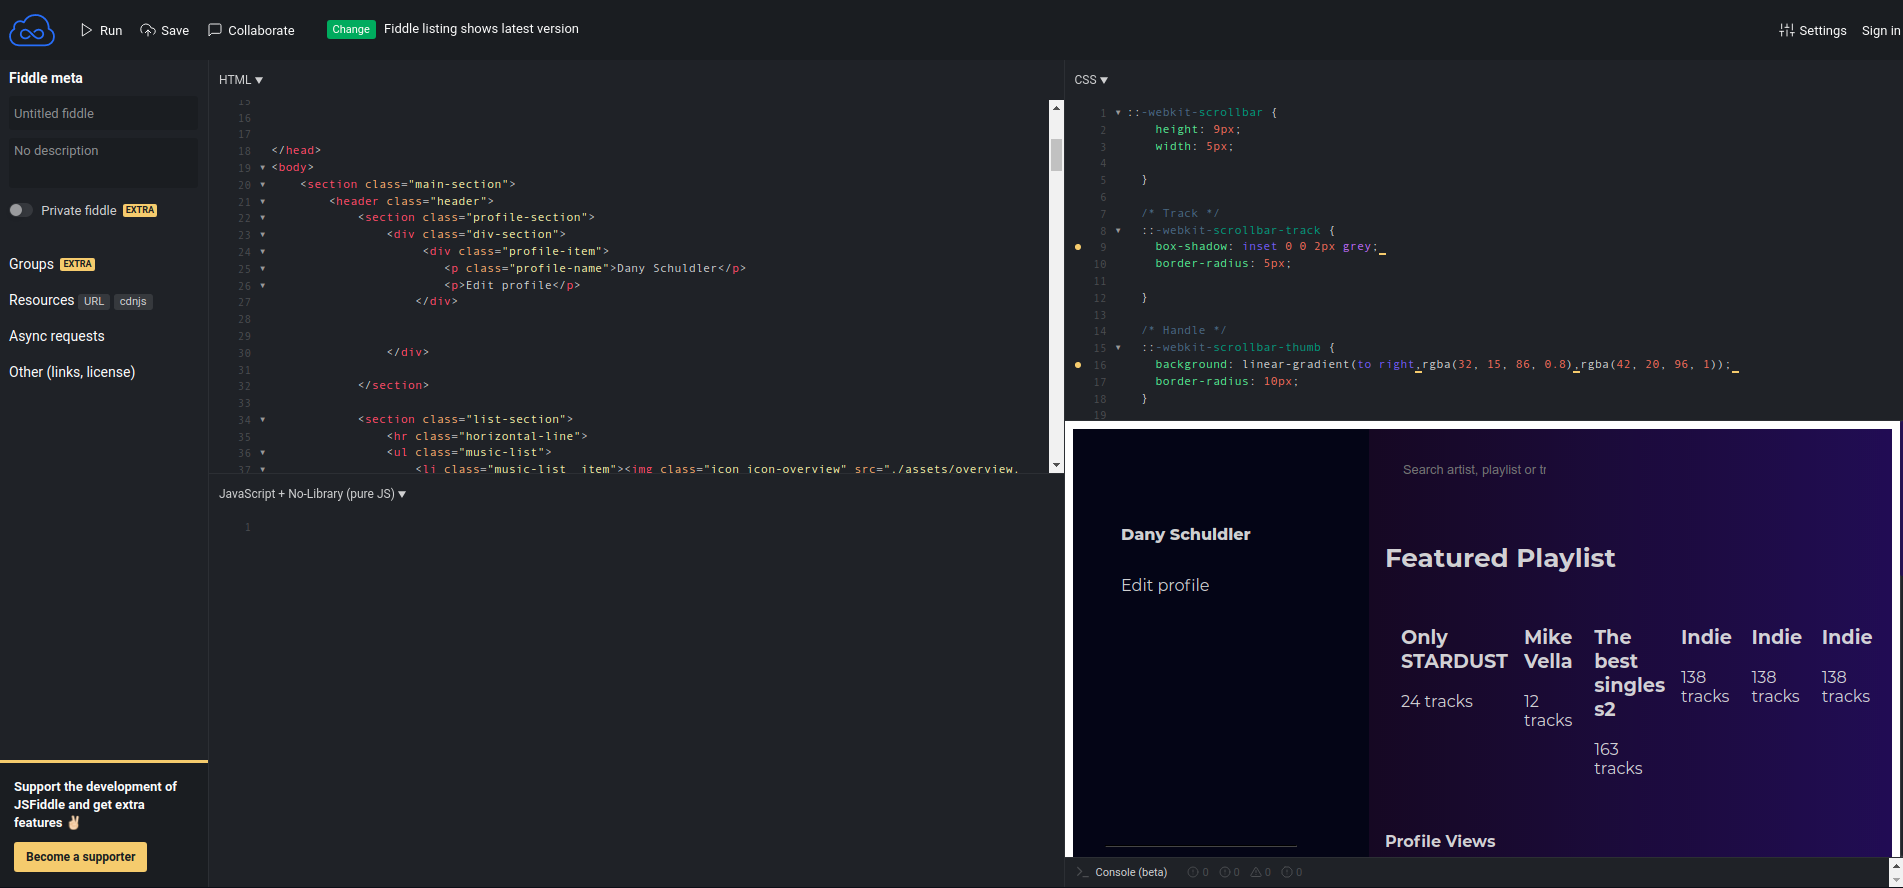
\includegraphics[width=0.9\linewidth]{Pictures/JS_Fiddle_Image}
	\caption{}
	\label{fig:jsfiddleimage}
\end{figure}



   